\input ../preamble

\begin{document}

{\Huge
  
  \centerline{\bf TTIC 31230, Fundamentals of Deep Learning}
  \bigskip
  \centerline{David McAllester, Winter 2018}
  \vfill
  \vfill
  \centerline{Multiclass Logistic Regression}
  \vfill
  \centerline{Multilayer Perceptrons (MLPs)}
  \vfill
  \centerline{Stochastic Gradient Descent (SGD)}
  \vfill
  \vfill

\slide{Multiclass Classification}

We consider the problem of taking an input $x$ (such as an image of a hand written digit) and classifying it into some small number of classes (such as the digits $0$ through $9$).

\vfill
\centerline{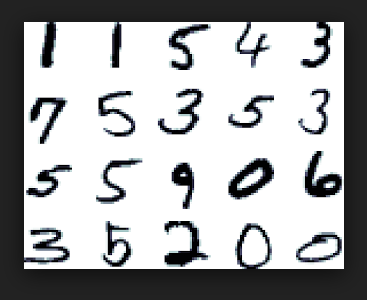
\includegraphics[width= 4.0in]{../images/MNIST}}
  
\slide{Multiclass Classification}

Assume a population distribution on pairs $(x,y)$ for $x \in \reals^d$ and $y \in {\cal C}$.

\vfill
For MNIST $x$ is a $28 \times 28$ image which we take to be a 784 dimensional vector giving $x \in \reals^{784}$.

\vfill
For MNIST ${\cal C}$ is the set $\{0,\ldots,9\}$.

\vfill
Assume a sample $(x_0,y_0),\;\ldots,\;(x_{N-1},y_{N-1})$ drawn IID from the population.

\vfill
We want to use the sample to construct a rule for predicting $y$ given $x$ when we draw new pairs from the population.

\slide{Multiclass Logistic Regression}

Assume a sample $(x_0,y_0),\;\ldots,\;(x_{N-1},y_{N-1})$ drawn IID from the population with $x \in \reals^d$ and $y \in \{0,\ldots,K\}$.

\vfill
For a new $x$ we compute a score $s(\hat{y})$ for each possible label $\hat{y}$.

\vfill
$$s = Wx + b$$

\slide{Multiclass Logistic Regression for MNIST}

$j$ --- image pixel

\vfill
$\hat{y}$ --- possible image label (0 through 9)

\vfill
$$s(\hat{y}) = \sum_j W[\hat{y},j]\; x[j] + b[\hat{y}]$$

\vfill
Note that $W[\hat{y},:]$ is an image.

\slide{Softmax}

Softmax converts scores (or energies or logits) to probabilities.

\vfill
\begin{eqnarray*}
  Q(\hat{y}) & = & \frac{1}{Z}\; e^{s(\hat{y})}
  \\
  \\
  \\
  Z & = & \sum_{\hat{y}} e^{s(\hat{y})}
\end{eqnarray*}

\vfill
In vector notation
\bigskip
$$Q  = \softmax\; s$$

\slide{Log Loss and Logistic Regression}
Let $Q_\Phi(\hat{y}|x)$ be defined by a model with parammeters $\Phi$.

\vfill
In logistic regression $\Phi$ is the pair $(W,b)$.

\vfill
Let $n$ range over training instances.

\begin{eqnarray*}
  W^*, b^* & = & \argmin_{W,b}\; \frac{1}{N} \sum_{n = 1}^N\;\;- \log Q_{W,b}(y_n|x_n) \\
  \\
  \\
  \Phi^* & = & \argmin_\Phi \;\frac{1}{N} \sum_{n = 1}^N\;\;- \log Q_\Phi(y_n|x_n) \\
\end{eqnarray*}


\slide{Information Theoretic Formulation}

Let $\Phi$ be the parameters of a probabilistc predictor $Q_\Phi$.

\vfill
\vfill
\centerline{We want \hspace{3ex} $\Phi^* = \argmin_\Phi \;\;\expectsub{(x,y) \sim {\cal P}}{ -\log Q_\Phi(y|x)}$.}

\vfill
\vfill
\vfill
This is {\bf cross-entropy} loss:

$$H({\cal P},{\cal Q}) = \expectsub{y \sim {\cal P}}{-\log\; {\cal Q}(y)}$$

$$H({\cal P}) = H({\cal P},{\cal P}) = \expectsub{y \sim {\cal P}}{-\log\; {\cal P}(y)}$$

$$H({\cal P},{\cal Q}) \geq H({\cal P})$$

$$\expectsub{(x,y) \sim {\cal P}}{ -\log Q_\Phi(y|x)} = \expectsub{x \sim {\cal P}}{H({\cal P}(:|x),Q_\Phi(:|x))}$$

\slide{Multi Layer Perceptrons (MLPs)}

Activation functions:
$$\sigma(u) = \frac{1}{1+e^{-u}}\;\;\;\;\;\;\;\;\mathrm{Relu}(u) = \max(u,0)$$

\vfill
\centerline{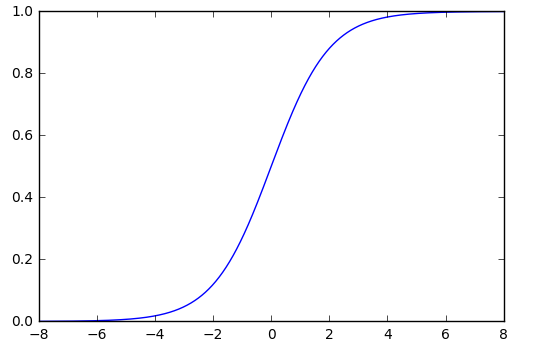
\includegraphics[width=1.5in]{../images/sigmoid}\hspace{1.0in}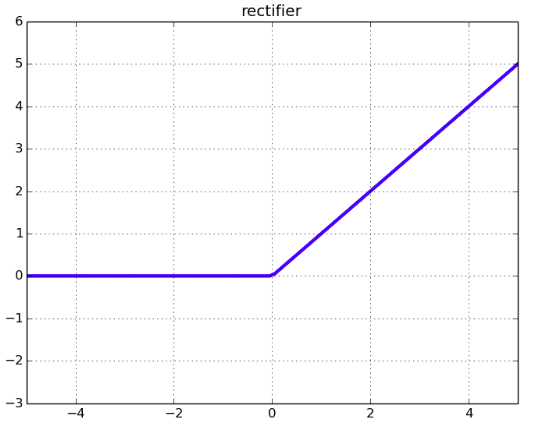
\includegraphics[width=1.2in]{../images/relu}}

\vfill
\begin{eqnarray*}
  L^0 & = & \mathrm{Relu}(W^0 x + b^0) \\
  \\
  L^1 & = & \sigma(W^1 L^0 + b^1) \\
  \\
  Q_\Phi & = & \softmax(L^1)
\end{eqnarray*}

\slide{Explicit Index Notation with {\em Typed Index Variables}}


$i$ --- pixels

$j$ --- image features

$\hat{y}$ --- possible image labels

\vfill
\begin{eqnarray*}
  L^0[j] & = & \mathrm{Relu}\left(\left(\sum_i\;W^0[j,i] \;x[i]\right) + b^0[j]\right) \\
  \\
  L^1[\hat{y}] & = & \sigma\left(\left(\sum_j\;W^1[\hat{y},j]\;L^0[j]\right) + b^1[\hat{y}]\right) \\
  \\
  Q_\Phi(\hat{y}) & = & \frac{1}{Z} \;e^{L^1[\hat{y}]}
\end{eqnarray*}

\ignore{
\slide{Index Types are Too Often Ignored}
For example: in Goodfellow et al. we have:


\centerline{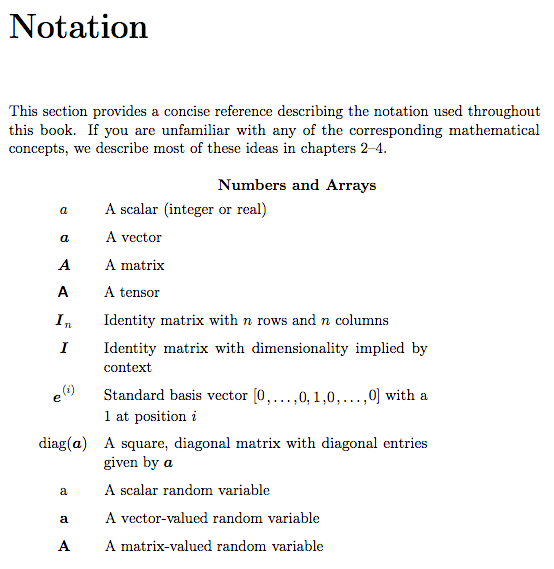
\includegraphics[height=5in]{../images/Notation}}

\slide{Abstract Optimization Problems}

Training minimizes (perhaps regularized) loss on the training data.

\vfill
$$\Phi^* = \argmin_\Phi\;\frac{1}{N} \sum_n \ell(\Phi,x_n,y_n)$$

\vfill
We would really like to minimize loss on the population.

\vfill
\vfill
$$\Phi^* = \argmin_\Phi\; E_{(x,y) \sim {\cal P}}\;\;\ell(\Phi,x,y)$$
}

\slide{Loss Vs. Error Rate}
While training (gradient descent) is generally done on log loss, performance is often judged by other measures such as error rate.

\vfill
The ``loss'' is often used as a synonym for log loss (or whatever loss defined the gradient descent training).

\vfill
Hence one often reports both ``loss'' and ``error rate''.

\vfill
Note that error rate is not differentiable.

\slide{Train Data, Development Data and Test Data}

Data is typically divided into {\bf a training set}, {\bf a development set} and {\bf a test set} each drawn IID from the population.

\vfill
A learning algorithm optimizes training loss.

\vfill
One then optimizes algorithm design (and hyper-parameters) on the development set. (graduate student descent).

\vfill
Ultimate performance should be done on a test set not used for development.  Test data is often withheld from developers.

\slide{Gradients with Respect to Systems of Parameters}

$\nabla_\Phi\;\ell(\Phi,x,y)$ denotes the partial derivative of $\ell(\Phi,x,y)$ with respect to the parameter system $\Phi$.

\vfill
Here can think of $\Phi$ as a single vector with
$$(\nabla_\Phi \;\ell(\Phi,x,y))_i = \partial \ell(\Phi,x,y) /\partial \Phi_i$$

\vfill
But in general $\Phi$ can be a multi-dimensional array (an ndarray in NumPy). If $\Phi$ is four dimensional we can write $\Phi[i,j,k,l]$.

\vfill
For scalar loss, $\nabla_\Phi \;\ell(\Phi,x,y)$ has the same shape as $\Phi$.

\vfill
$$\left(\nabla_\Phi \;\ell(\Phi,x,y)\right).\mathrm{shape} = \Phi.\mathrm{shape}$$

\slide{Total Gradient Descent}

$$\ell_{\mathrm{train}}(\Phi) = \frac{1}{N}\sum_n \ell(\Phi,x_n,y_n)$$

\vfill
\centerline{We want: \hspace{3ex} $\Phi^*  =  \argmin_\Phi \ell_{\mathrm{train}}(\Phi)$}

\vfill
$$\Phi \;\;\;\mbox{\tt -=}\;\;\; \eta \nabla_\Phi \ell_\mathrm{train}(\Phi)$$

\slide{Stochastic Gradient Descent (SGD) on the training set.}

\vfill
\vfill
repeat:  Select $n$ at random. $\Phi \;\;\minuseq\;\; \eta \;\nabla_\Phi \; \ell(\Phi,x_n,y_n)$

\begin{eqnarray*}
  \expectsub{n}{\nabla_\Phi \; \ell(\Phi,x_n,y_n)} & = & \sum_n P(n) \nabla_\Phi\;\ell_{\mathrm{train}}(\Phi,x_n,y_n) \\
  \\
  \\ & = & \frac{1}{N} \sum_n \nabla_\Phi\;\ell_{\mathrm{train}}(\Phi,x_n,y_n) \\
  \\
    \\ & = & \nabla_\Phi \frac{1}{N} \sum_n \;\ell_{\mathrm{train}}(\Phi,x_n,y_n) \\
  \\
  &  = & \nabla_\Phi\;\ell_{\mathrm{train}}(\Phi)
\end{eqnarray*}



\slide{Epochs}

In practice we cycle through the training data visiting each training pair once.

\vfill
One pass through the training data is called an Epoch.

\vfill
One typically imposes a random suffle of the training data before each epoch.

\slide{SGD for MLPs}

\centerline{$j$: feature \hfill $\ell$: layer \hfill $\hat{y}$: possible label}

\vfill
\begin{eqnarray*}
  L^0[j] & = & \mathrm{Input} \\
  \\
  L^{\ell+1}[j'] & = & \sigma\left(\left(\sum_j\;W^{\ell+1}[j',j]\;L^{\ell+1}[j]\right) + b^{\ell+1}[j']\right) \\
  \\
  L^N[\hat{y}] & = & \sigma\left(\left(\sum_j\;W^{N-1}[\hat{y},j]\;L^{N-1}[j]\right) + b^{N-1}[\hat{y}]\right) \\
  \\
  \\
  P(\hat{y}) & = & \frac{1}{Z} \;e^{L^N[\hat{y}]}
\end{eqnarray*}


\slideplain{END}
}
\end{document}
